\documentclass{beamer}
\usetheme{Boadilla}
\usepackage[utf8x]{inputenc}
\usepackage{listings}
\usepackage{subfig}
%\title{LS Genio Platform}
%\subtitle{Piattaforma per il monitoraggio di macchine utensili con integrazione a software ERP Microsoft Dynamics NAV}
%\author{Vincenzo Nucci e Matteo Tiberi}
%\author{Matteo Tiberi}
%\institute{Università di Camerino}
\date{}
\begin{document}
	
	\begin{frame}
	\centering
	
\includegraphics[scale=0.25]{images/frontespizio-beamer.png}\par
	\usebeamertemplate{title page}
\end{frame}

\begin{frame}
	\frametitle{Sommario}
	Obiettivo di questa tesi è stato la realizzazione di una piattaforma REST che restituisca misurazioni fatte da sensori collegati a macchinari utensili. La natura delle misurazioni è descritta da una ontologia. Parte del progetto è stata l'integrazione di questi servizi con il gestionale NAV. Infine la piattaforma deve visualizzare dati attraverso un grafico dinamico e poter applicare un controllo di superamento di una soglia. Tutti gli obiettivi prefissati sono stati raggiunti, affrontando piccole difficoltà implementative, grazie ai software utilizzati.
\end{frame}

\begin{frame}
\frametitle{Obiettivi}
\begin{itemize}
	\item Piattaforma REST indipendente da sorgenti dati
	\begin{itemize}
		\item Autenticazione tramite token
		\item Interfaccia web
	\end{itemize}
	\item Servizio di sottoscrizione "subscribe"
	\begin{itemize}
		\item Notifica dei messaggi PUSH
	\end{itemize}
	\item Integrazione dei servizi con NAV
	\item Servizio di monitoraggio dei dati
	\begin{itemize}
		\item Controllo valore oltre soglia
	\end{itemize}
\end{itemize}
\end{frame}

\begin{frame}
\frametitle{Architettura piattaforma}
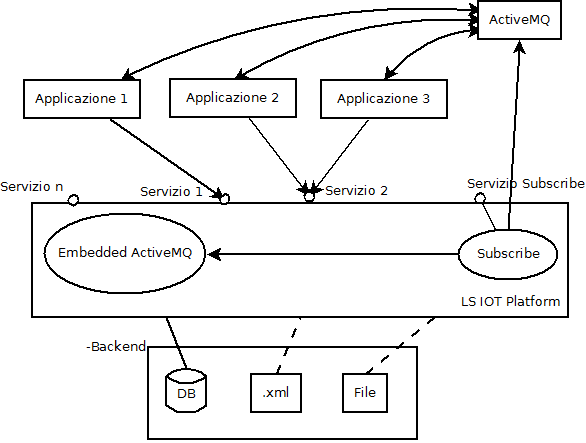
\includegraphics[width=0.9\textwidth]{images/architettura_piattaforma.png}
\end{frame}

\begin{frame}
\frametitle{Pagina catalogo Smart Object}
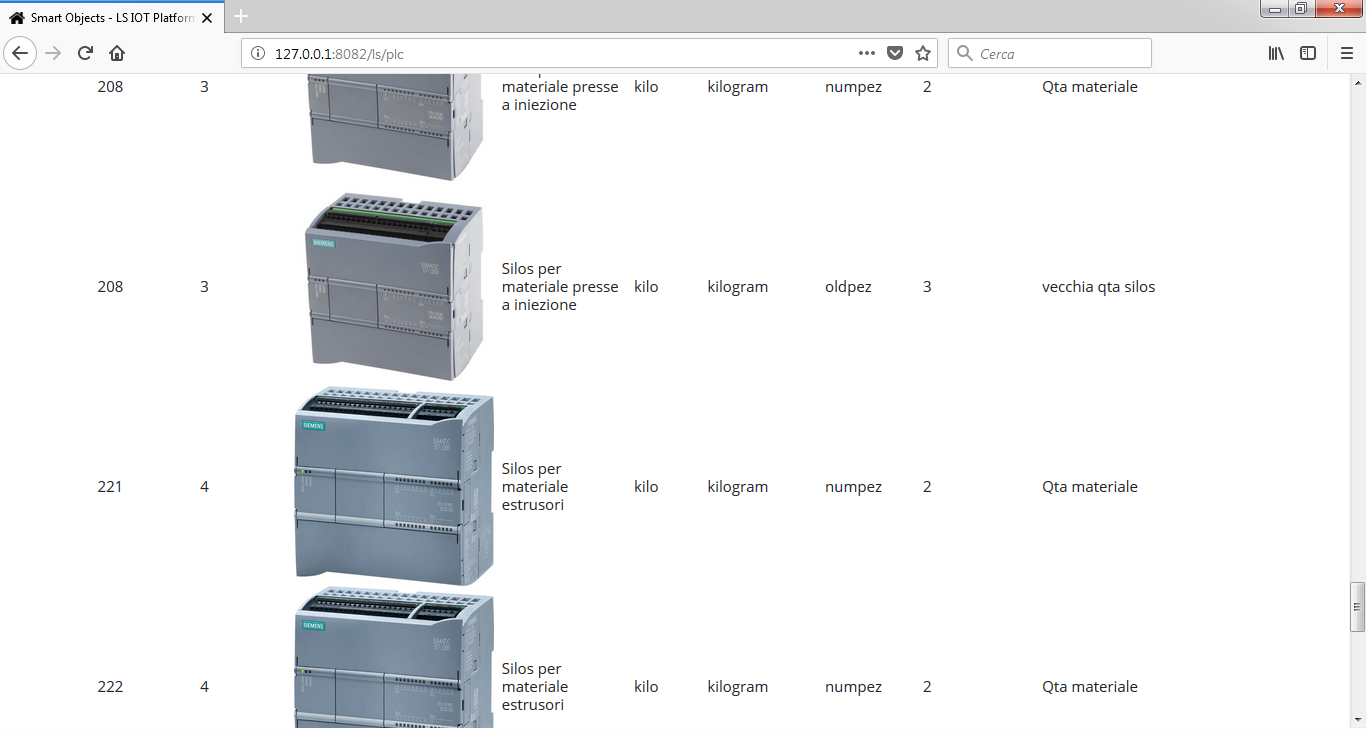
\includegraphics[width=1\textwidth]{images/SmartObjectsPlatform.png}
\end{frame}

\begin{frame}
\frametitle{Esempio valori di ritorno di un servizio}
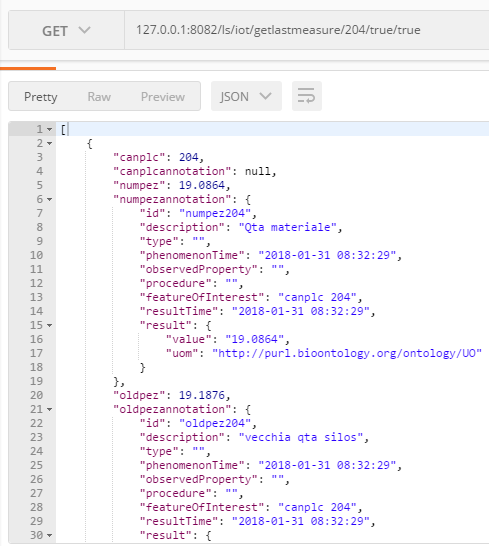
\includegraphics[width=0.6\textwidth]{images/Postman1.png}
\end{frame}

\begin{frame}
\frametitle{Subscribe Rule di una applicazione}
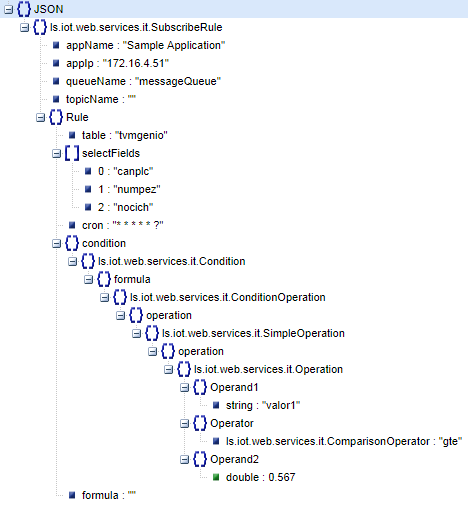
\includegraphics[width=0.6\textwidth]{images/subscribe-json-1.png}
\end{frame}

\begin{frame}
\frametitle{Pagina web per il grafico del monitoraggio}
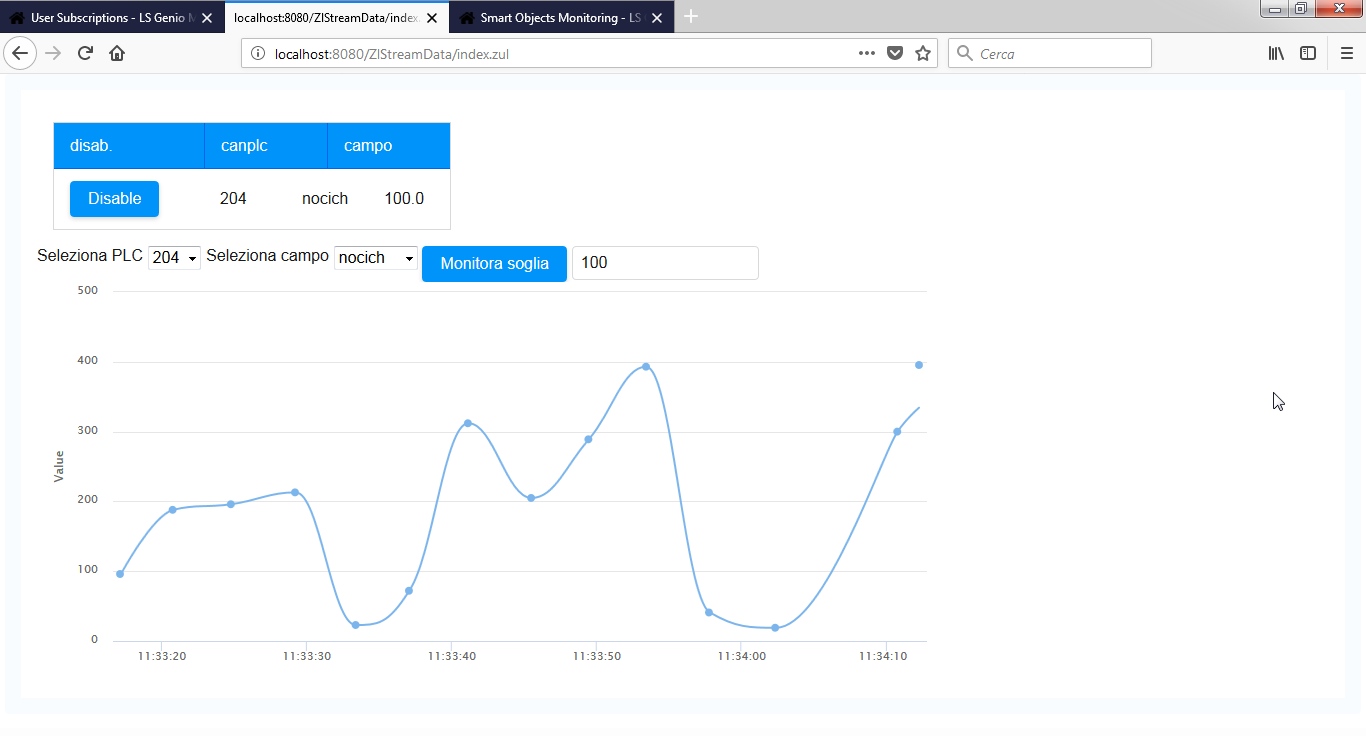
\includegraphics[width=1\textwidth]{images/grafico-zk.png}
\end{frame}

\begin{frame}
\frametitle{Codice Job Flink}
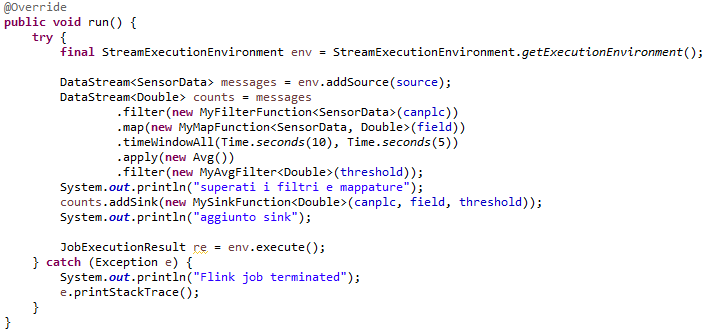
\includegraphics[width=1\textwidth]{images/flink-job.png}
\end{frame}

\begin{frame}
	\frametitle{Conclusioni}
	Questo progetto ha mostrato quanta innovazione e benefici porti alle aziende implementare le novità introdotte dall’Industria 4.0, tra le quali i Big Data rappresentano la componente principale.
\end{frame}

%-------------------------inizio client-----------------------------
\begin{frame}
\frametitle{Sommario}
La parte client è principalmente focalizzata sull’utilizzo dei servizi forniti dalla piattaforma LS-Genio Mashup con il software gestionale Microsoft Dynamics NAV e nella realizzazione di un ontologia delle misurazioni e misure dei dati restituiti (i quali sono relativi a misurazioni di sensori su macchine utensili). Su questi dati, inoltre, è stata realizzata una visualizzazione grafica visibile tramite il gestionale NAV.
\end{frame}

\begin{frame}
\frametitle{Obiettivi}
\begin{itemize}
	\item Interazione di Microsoft Dynamics NAV con la piattaforma LS-Genio Mashup e definizione di un "setup" per l'utente
	%\begin{itemize}
	%	\item Mancata possibilità di consumo diretto di servizi REST
	%	\item Mancata possibilità di gestione del formato JSON
	%	\item Difficoltà nell'interazione con software esterni non Microsoft
	%\end{itemize}
	
	%\item Visualizzazione tramite NAV di un report PowerBI basato sui dati ottenuti
	%\item Visualizzazione da NAV di una rappresentazione grafica con PowerBI dei dati ottenuti 
	\item Realizzazione di un ontologia delle misurazioni e delle misure
\end{itemize}	
\end{frame}

\begin{frame}
\frametitle{La pagina Machine Assignment List}
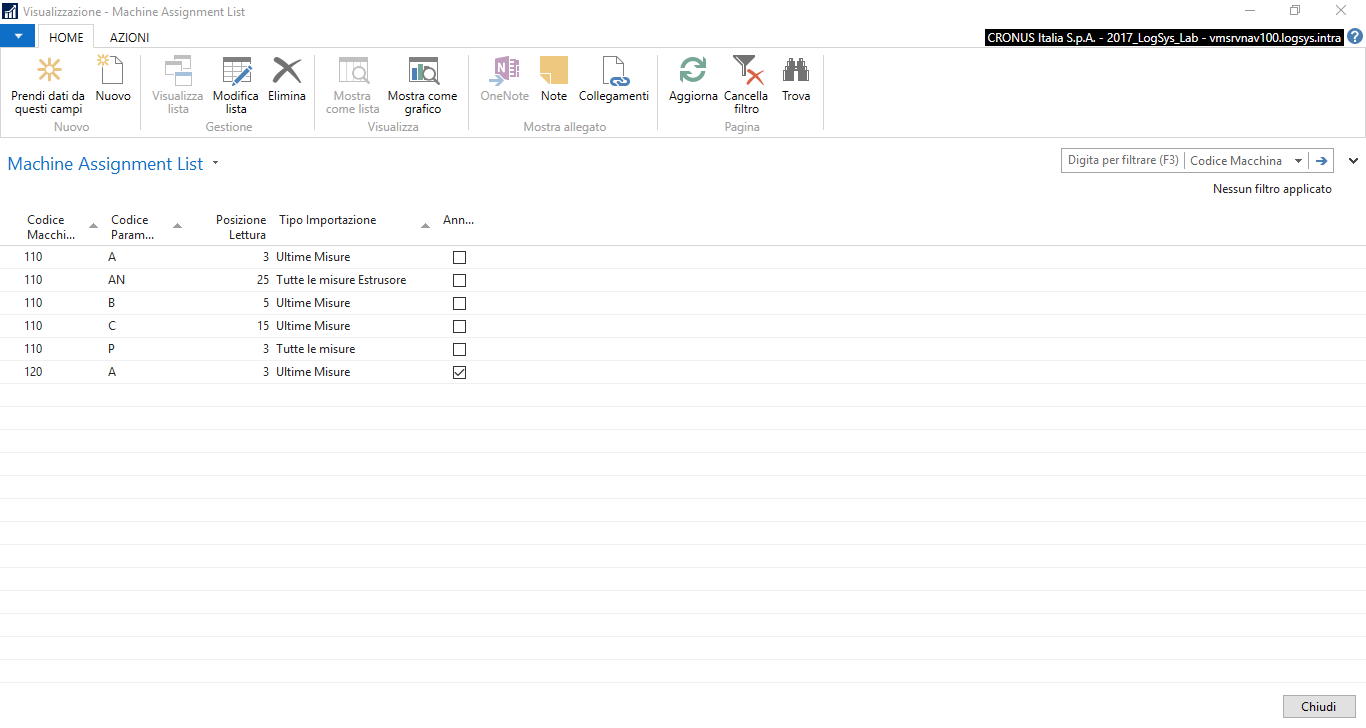
\includegraphics[width=1\textwidth]{images/MachineAssignmentList2.png}
\end{frame}


%\begin{frame}
%\frametitle{Lista con i parametri}
%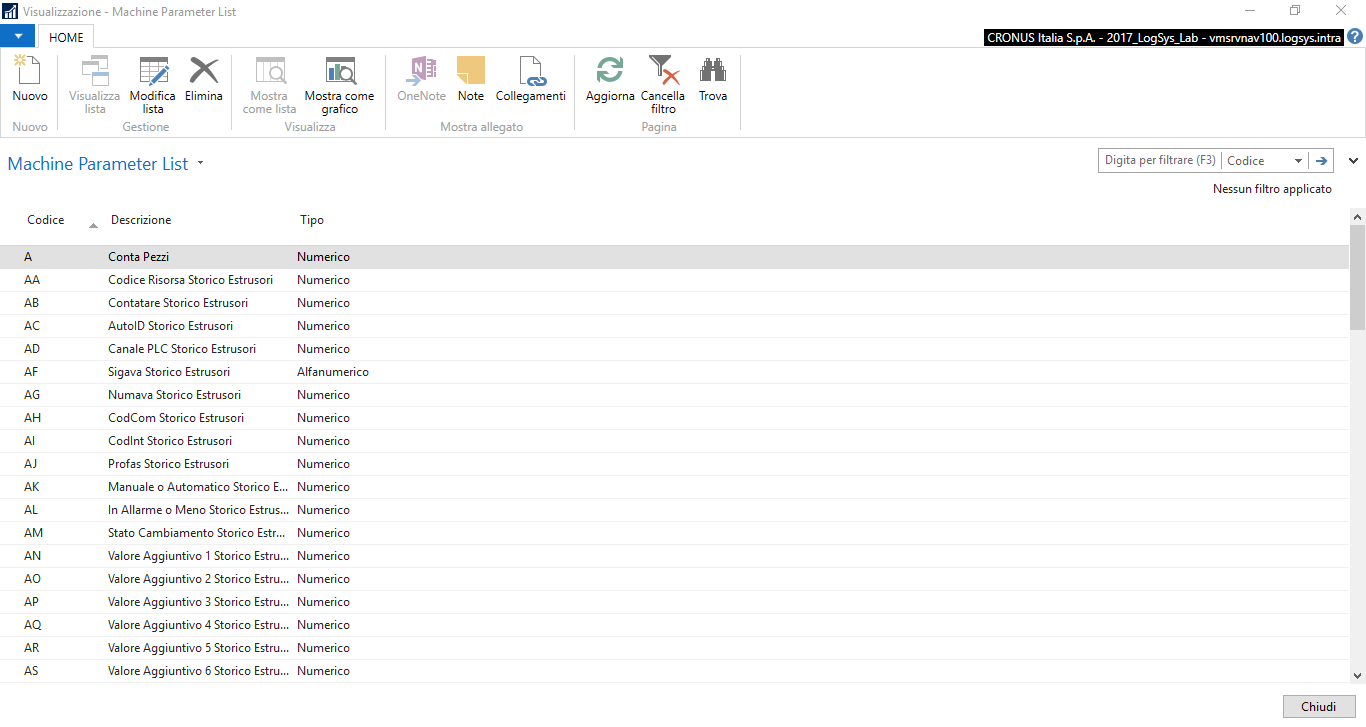
\includegraphics[width=1\textwidth]{images/MachineParameter.png}
%\end{frame}

%\begin{frame}
%\frametitle{Pagina del token}
%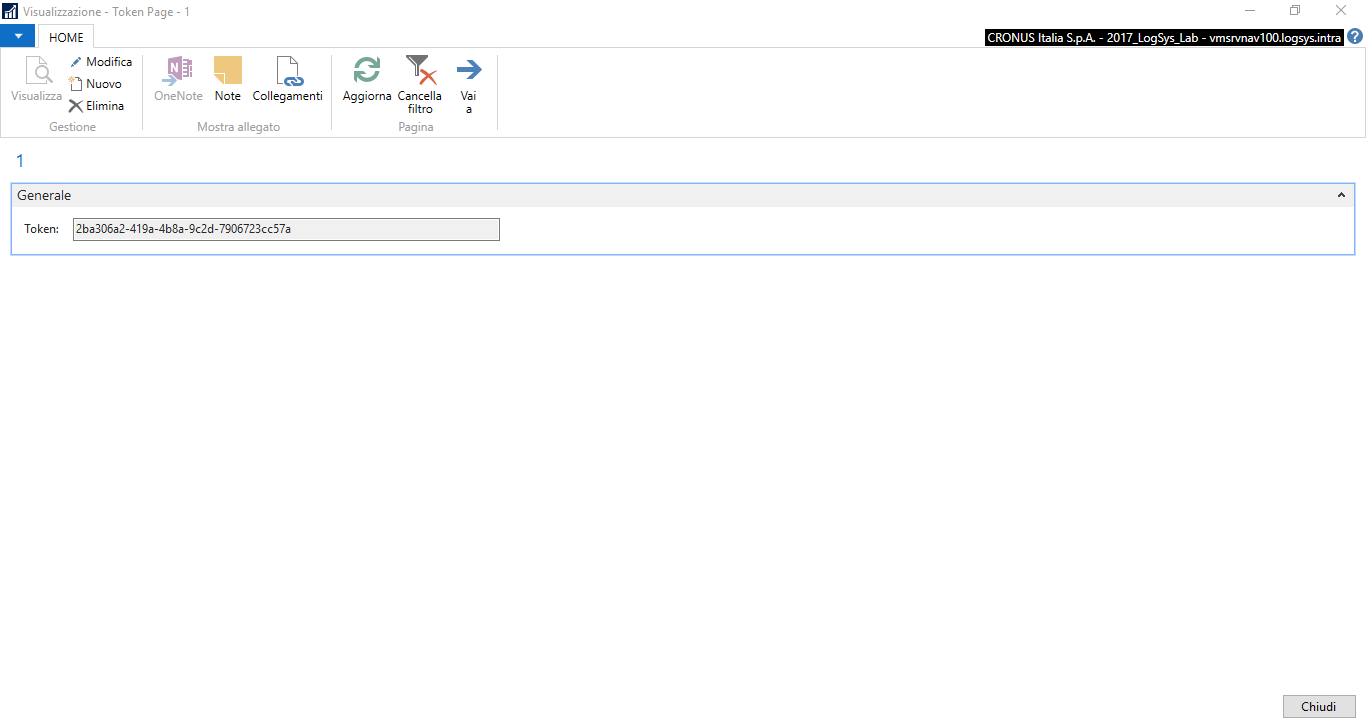
\includegraphics[width=1\textwidth]{images/tokenpage.png}
%\end{frame}



\begin{frame}
\frametitle{La pagina Machine Reading List}
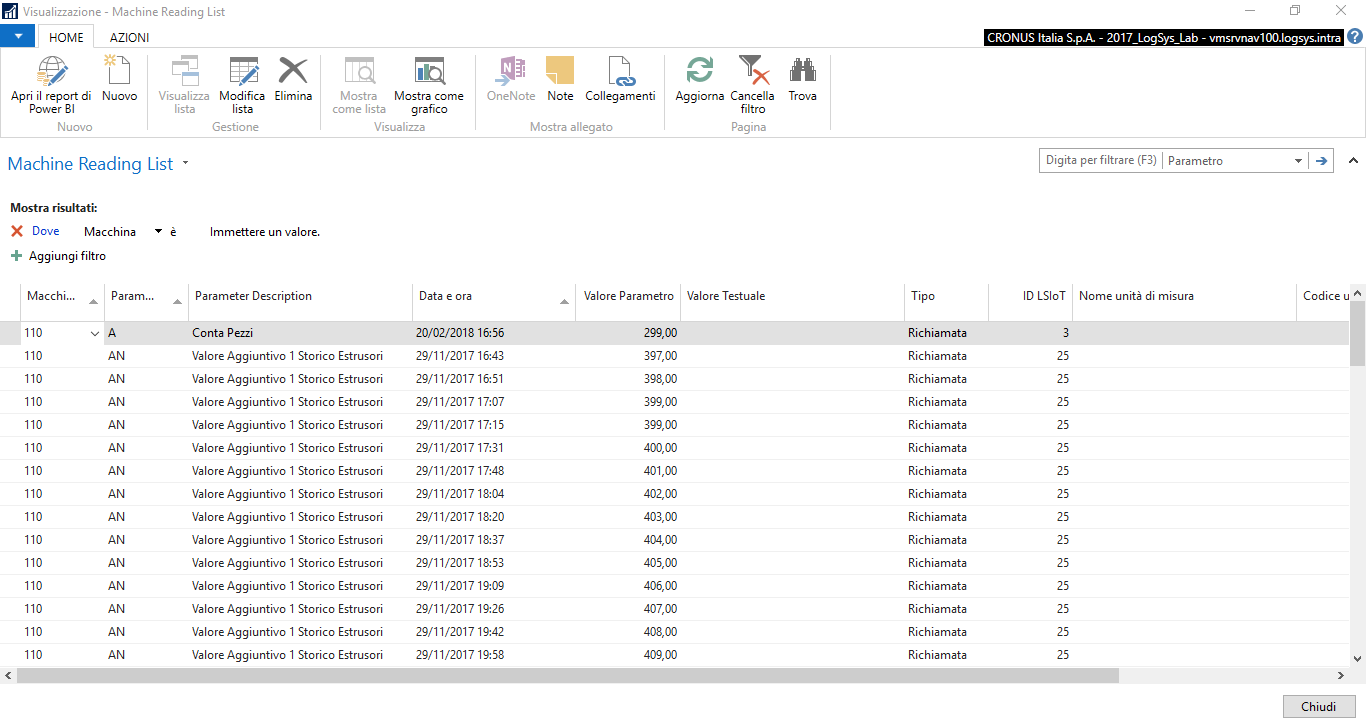
\includegraphics[width=1\textwidth]{images/MachineReadingList.png}
\end{frame}

%\begin{frame}
%\frametitle{Il report PowerBI nell'applicativo}
%\includegraphics[width=1\textwidth]{images/PowerBI.png}
%\end{frame}

\begin{frame}
\frametitle{Il report PowerBI esportato nel web}
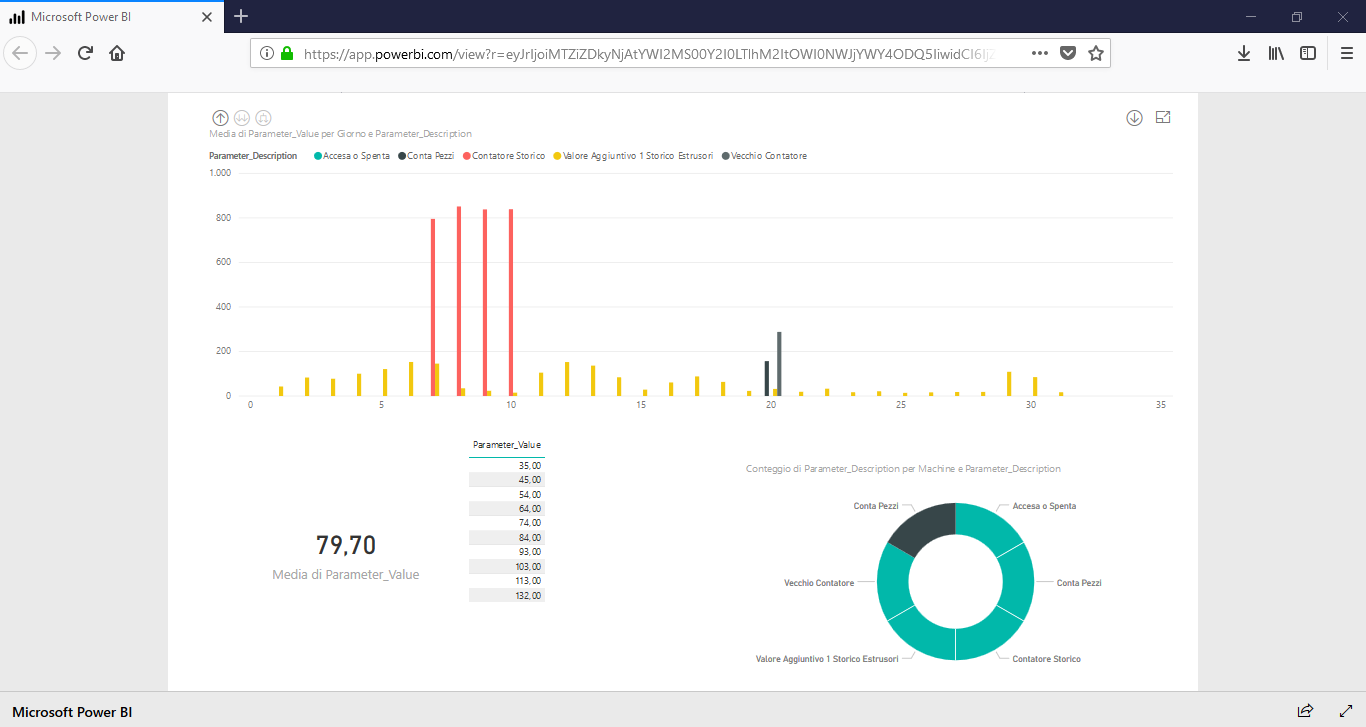
\includegraphics[width=1\textwidth]{images/ReportWEB.png}
\end{frame}

%\begin{frame}
%\frametitle{Metodo SetMeasurementPLC}
%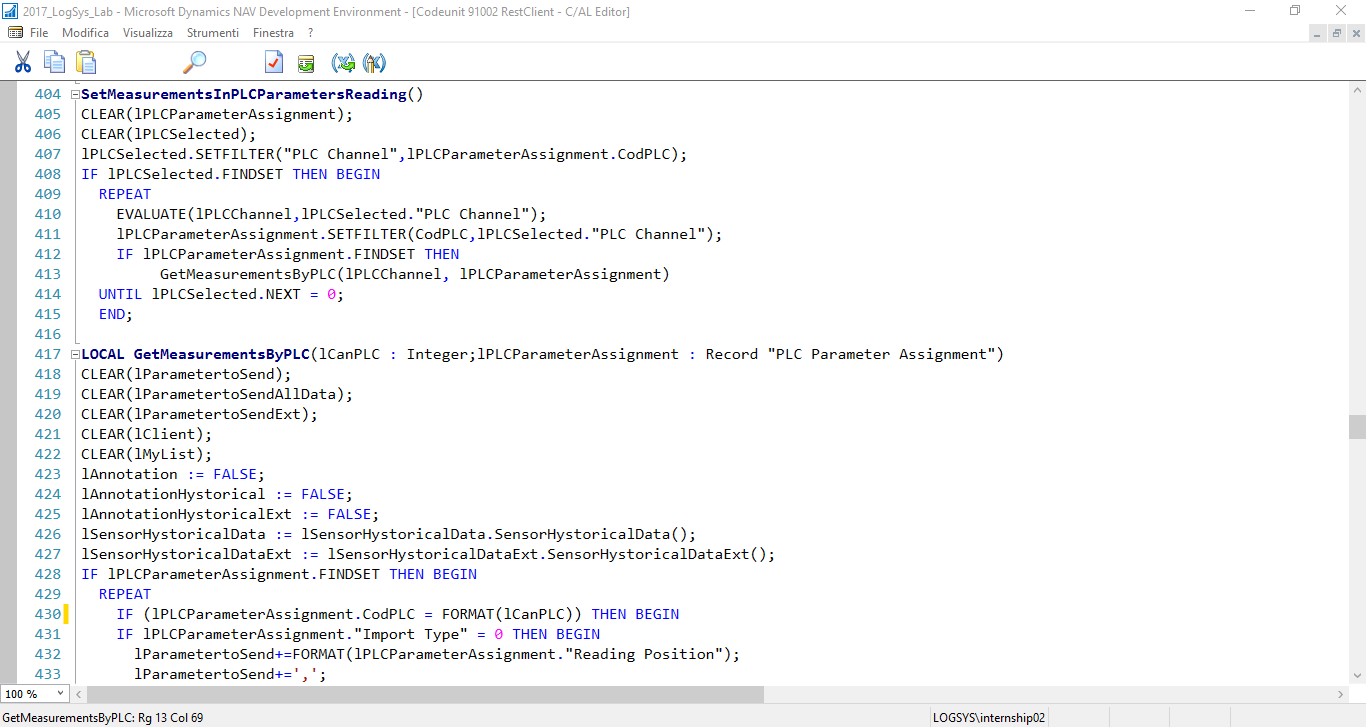
\includegraphics[width=1\textwidth]{images/NAVSetMesurament.png}
%\end{frame}

%\begin{frame}
%\frametitle{Metodo GetMeasurementPLC1}
%\includegraphics[width=1\textwidth]{images/NAVGetMesurament1.png}
%\end{frame}

%\begin{frame}
%\frametitle{Metodo GetMeasurementPLC2}
%\includegraphics[width=1\textwidth]{images/NAVGetMesurament2.png}
%\end{frame}

%\begin{frame}
%\frametitle{NAV servizi web}
%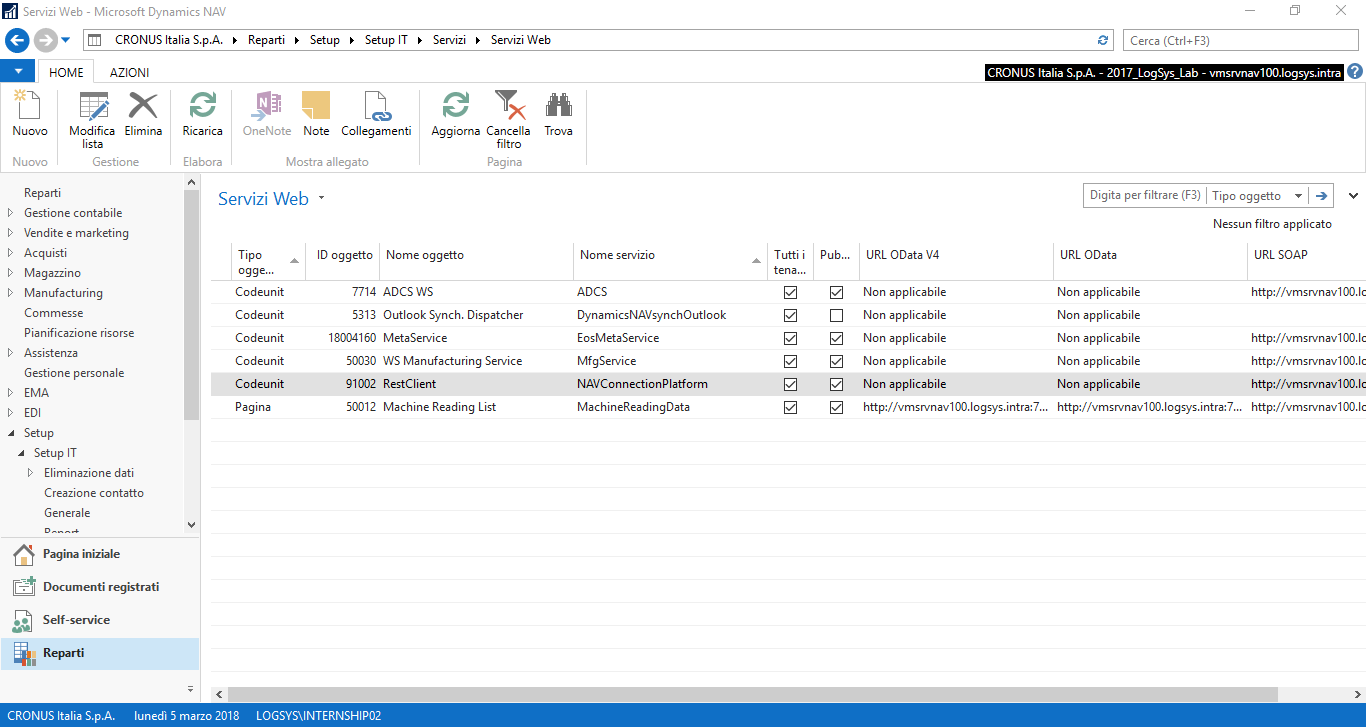
\includegraphics[width=1\textwidth]{images/NAVServiziWeb.png}
%\end{frame}


%\begin{frame}
%\frametitle{NAV SubscriptionPage}
%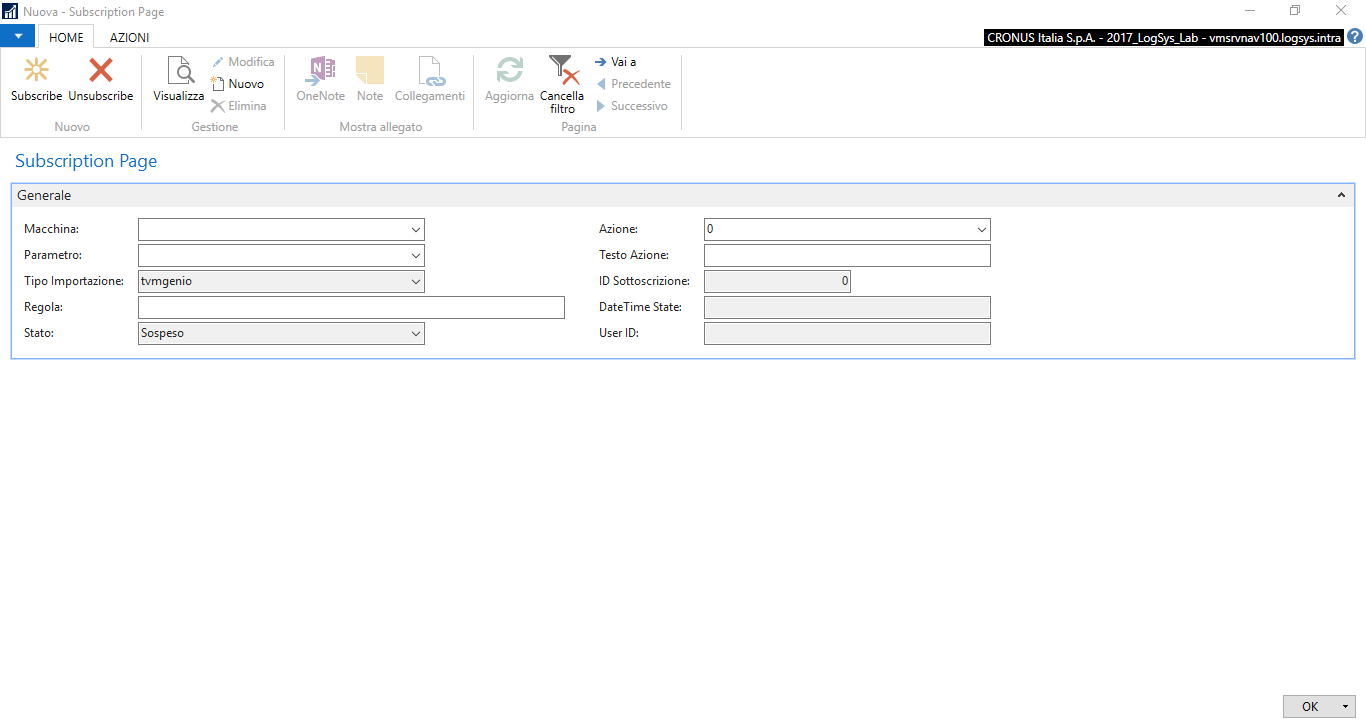
\includegraphics[width=1\textwidth]{images/NAVSubscriptionPage.png}
%\end{frame}

\begin{frame}
\frametitle{Standard Observation and Measurement ISO 19156:2011}
\begin{itemize}
\item Standard basato sul concetto di osservazione, con implementazioni in formato XML e JSON
\begin{itemize}
\item Pensato per l'ambito geospaziale, il modello risulta astratto e applicabile nel case study
\end{itemize}
\item Concetto di osservazione generico specializzato in base al risultato (es. Measurement)
\begin{itemize}
%\item All'interno del case study non tutte le specializzazioni proposte vengono utilizzate
\item Solo alcune specializzazioni sono utilizzate nel case study
\end{itemize}
\item Al risultato di una osservazione specializzata viene poi associata un ontologia delle misure
\end{itemize}	
\end{frame}

%\begin{frame}
%\frametitle{Tabelle Annotazioni}
%\includegraphics[width=1\textwidth]{images/AltreTabelleAnnotazioniMOD4.png}
%\end{frame}

%\begin{frame}
%\frametitle{Metodo PushMeasurement 1}
%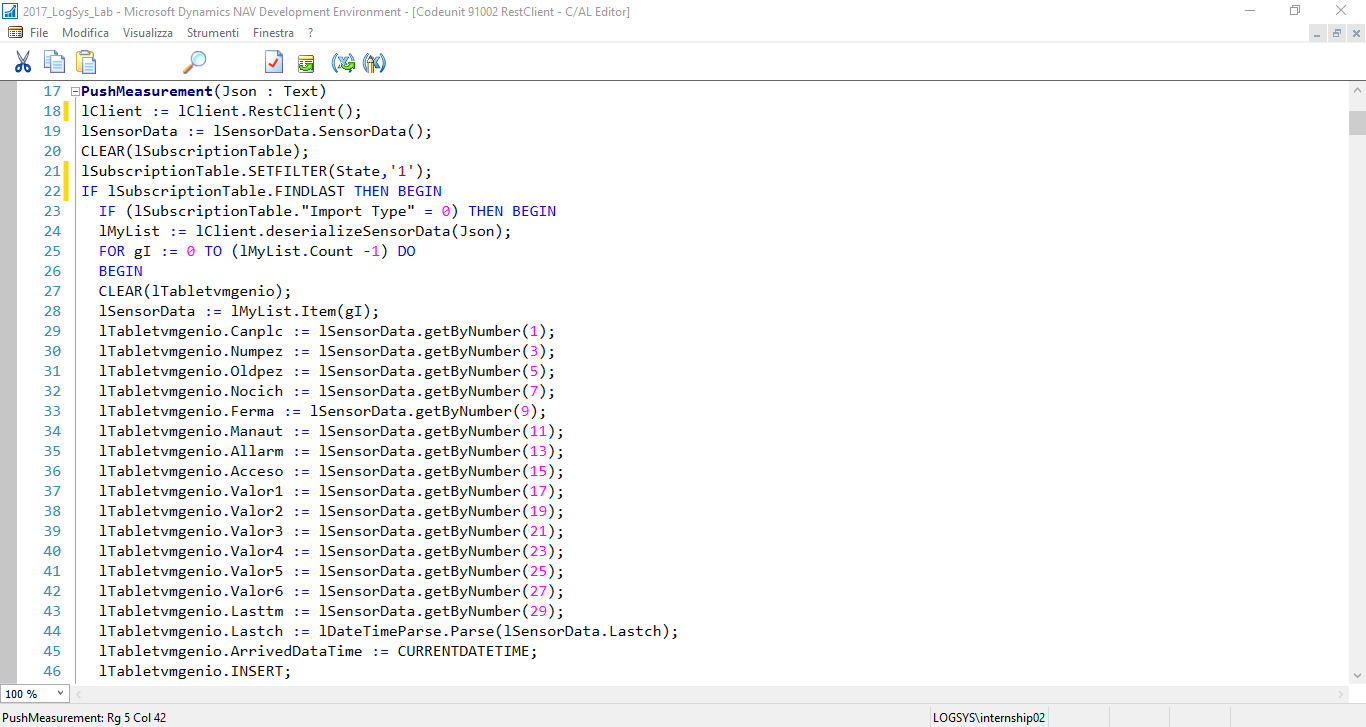
\includegraphics[width=1\textwidth]{images/NAVPushMeasuraments1.png}
%\end{frame}

%\begin{frame}
%\frametitle{Metodo PushMeasurement 2}
%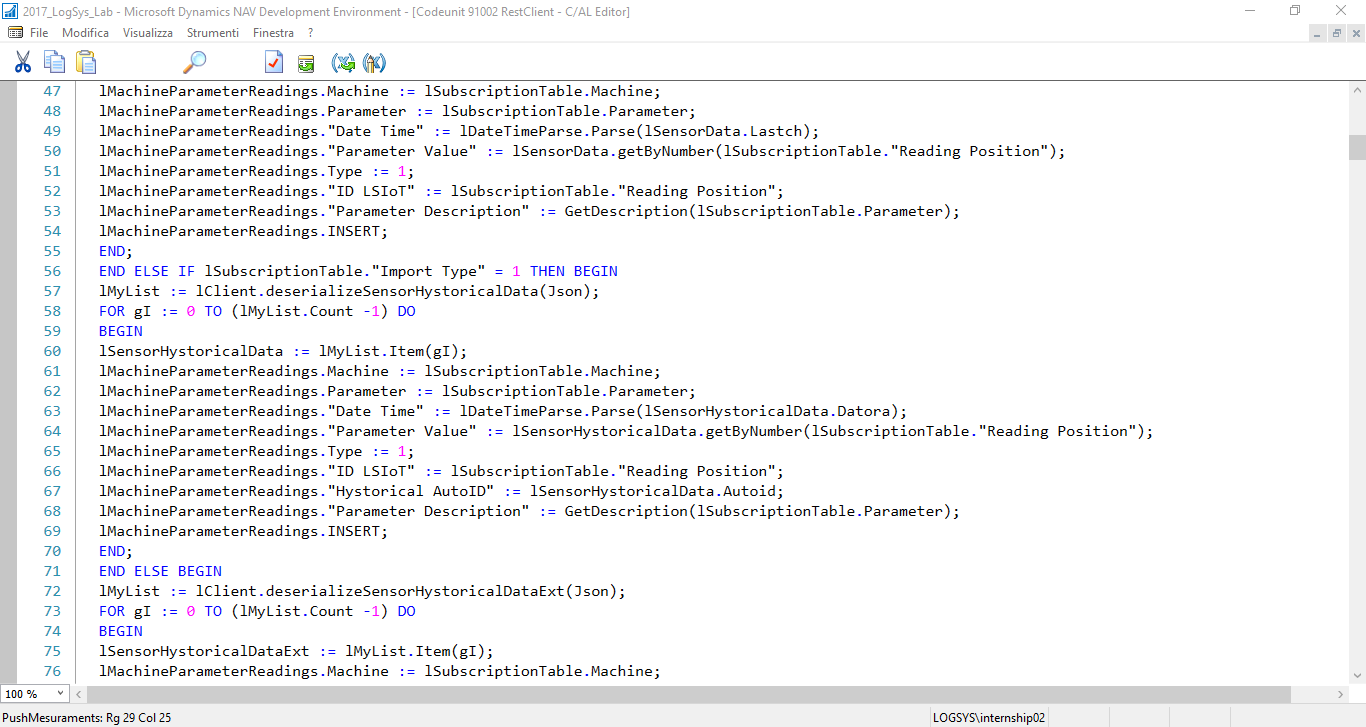
\includegraphics[width=1\textwidth]{images/NAVPushMeasuraments2.png}
%\end{frame}

%\begin{frame}
%\frametitle{Metodo PushMeasurement 3}
%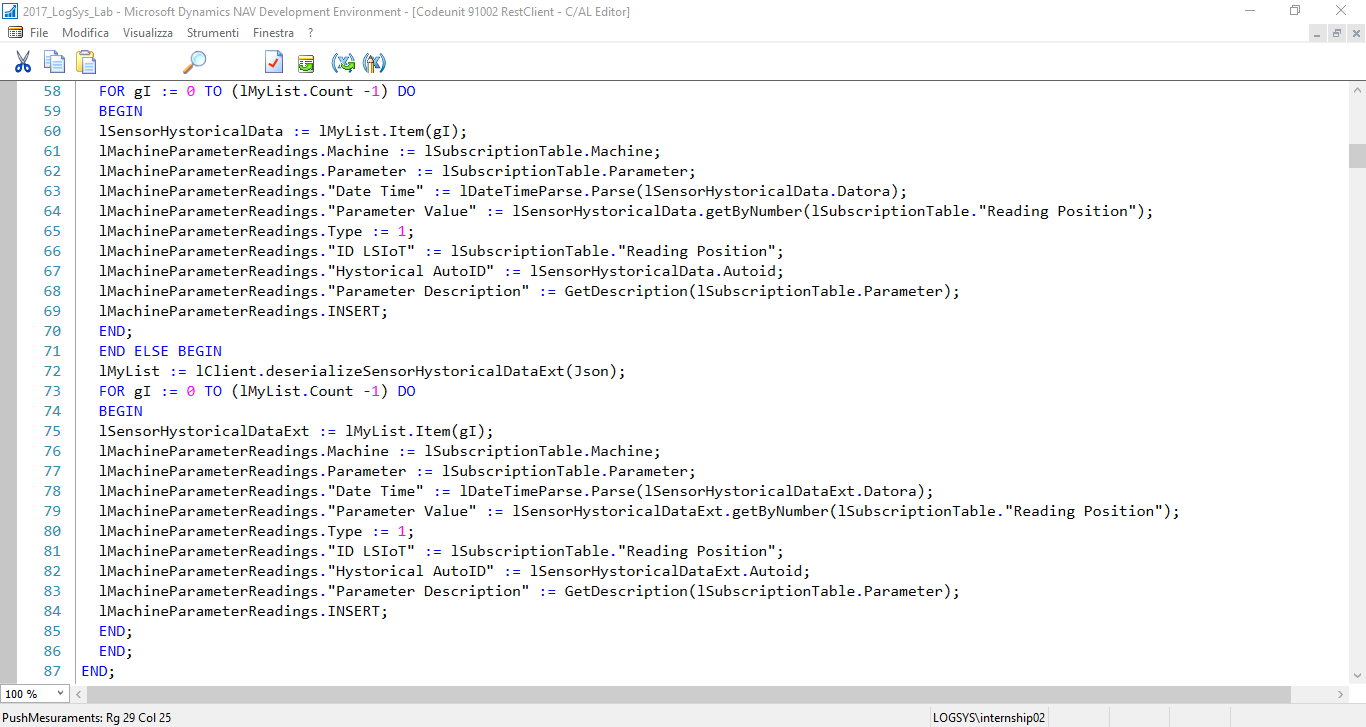
\includegraphics[width=1\textwidth]{images/NAVPushMeasuraments3.png}
%\end{frame}

%\begin{frame}
%\frametitle{Esempio XML}
%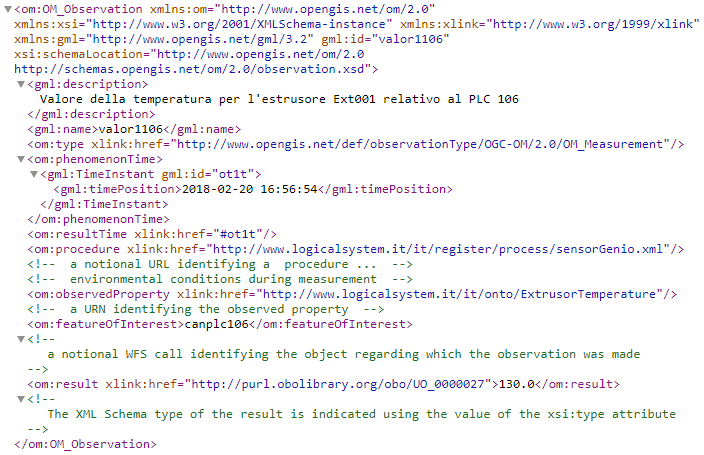
\includegraphics[width=1\textwidth]{images/TemperatureXML2.png}
%\end{frame}

\begin{frame}
\frametitle{Esempio JSON}
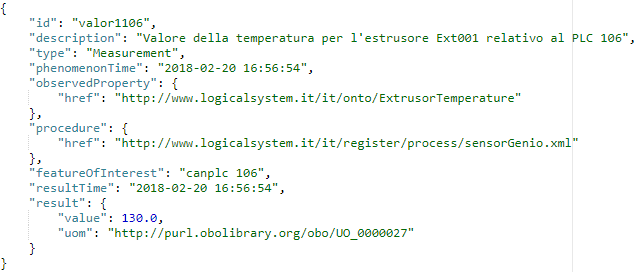
\includegraphics[width=1\textwidth]{images/TemperatureJSON.png}
\end{frame}

%\begin{frame}
%\frametitle{Grafico Misurazioni e misure}
%\begin{figure}%
%	\centering%
%	\subfloat{{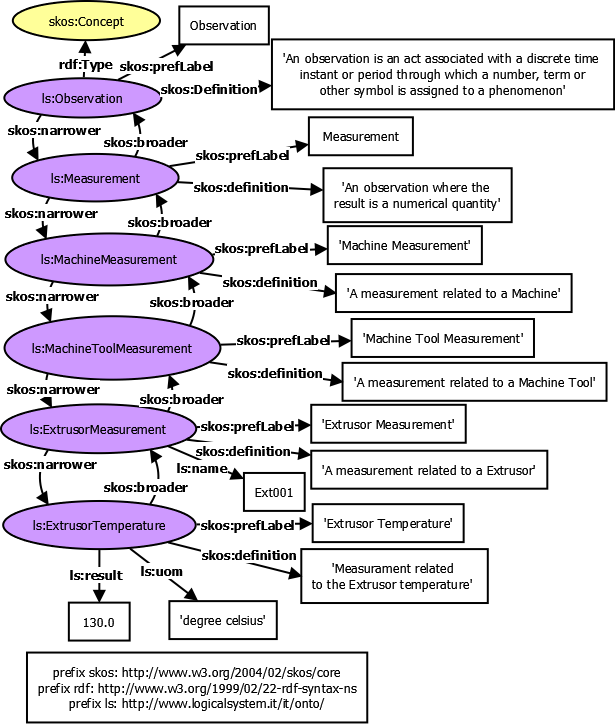
\includegraphics[width=6.84cm]{images/TempExample2.png} }}%
%	\qquad
%	\subfloat{{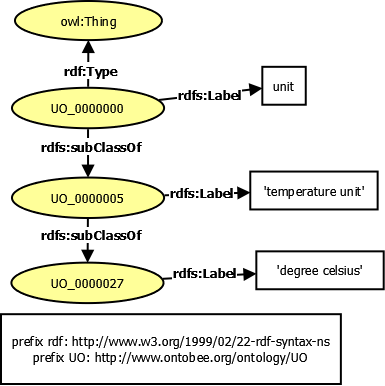
\includegraphics[width=4.7cm]{images/celsius.png} }}%
%
%
%\end{figure}
%\end{frame}

\begin{frame}
\frametitle{Grafico Misurazioni e misure}
\begin{figure}%
%\centering
\subfloat{{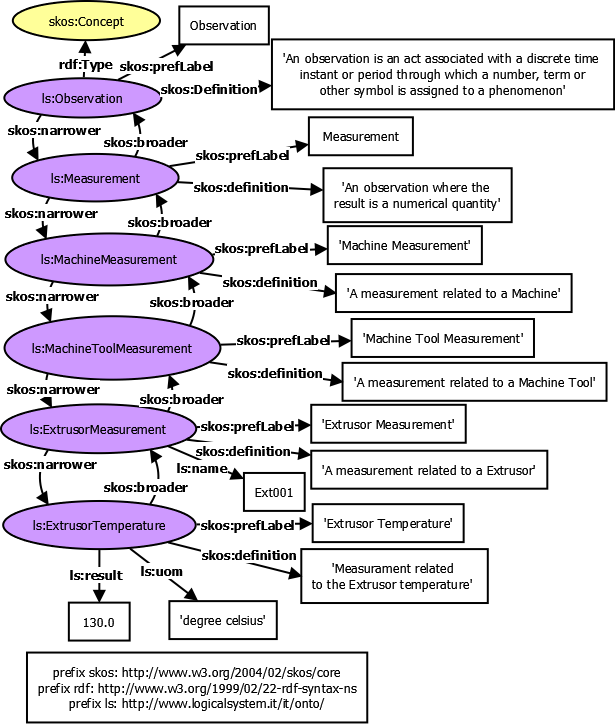
\includegraphics[width=0.565\columnwidth]{images/TempExample2.png} }}%
%\qquad
\hfill
\subfloat{{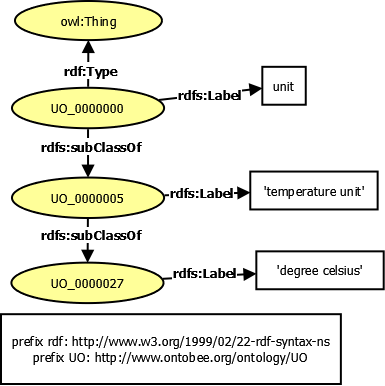
\includegraphics[width=5cm]{images/celsius.png} }}%
%
%
\end{figure}
\end{frame}


%\begin{frame}
%\frametitle{Grafico Misurazioni e misure 2}
%\begin{figure}
%	\subfigure[]{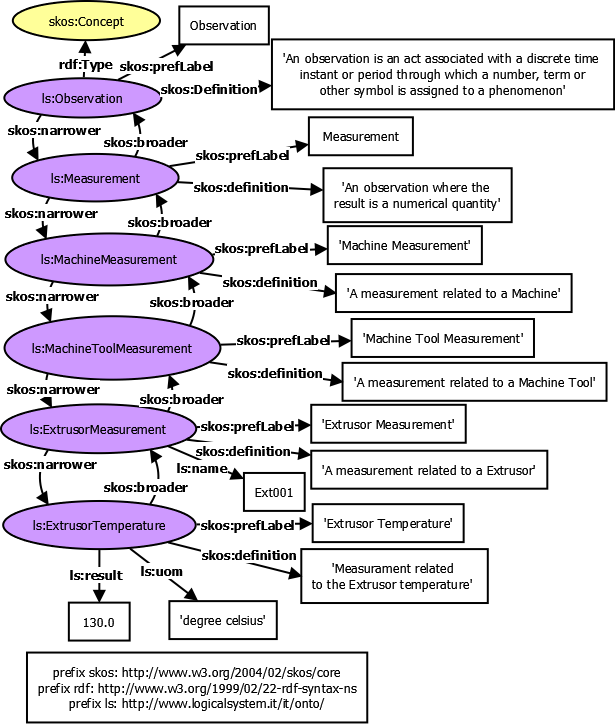
\includegraphics[width=7cm]{images/TempExample2.png}}
%	\hfill
%	\subfigure[]{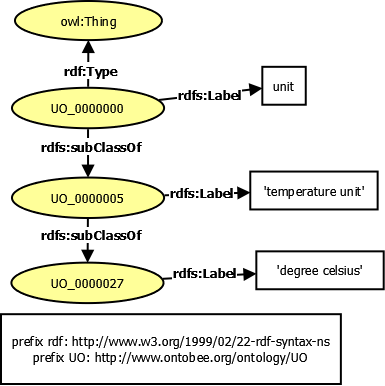
\includegraphics[width=4.7cm]{images/celsius.png}}
%\end{figure}
%\end{frame}

%\begin{frame}
%\frametitle{Grafico Misurazioni}
%\begin{center}
%	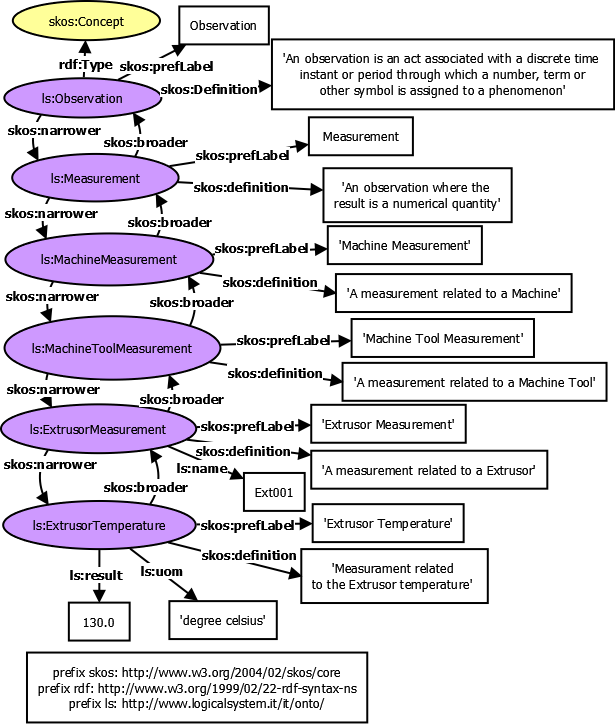
\includegraphics[width=0.6\textwidth]{images/TempExample2.png}
%\end{center}
%\end{frame}

%\begin{frame}
%\frametitle{Grafico Misure}
%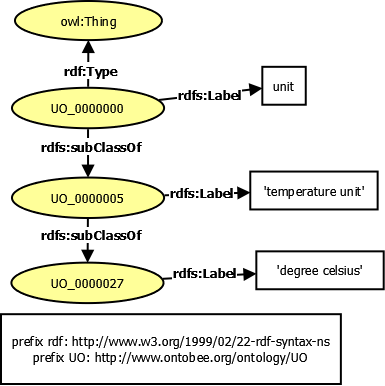
\includegraphics[width=0.6\textwidth]{images/celsius.png}
%\end{frame}

%\begin{frame}
%\frametitle{JSON con annotazione semantica}
%\includegraphics[width=1\textwidth]{images/JSONRestituito.png}
%\end{frame}

\begin{frame}
\frametitle{Conclusioni}
\begin{itemize}
\item L'integrazione tra NAV e la piattaforma ha avuto esito positivo tramite uso del client C\# 
\begin{itemize}
\item Permettendo agli utenti un semplice utilizzo dei servizi
\end{itemize}
%\item Il report PowerBI è disponibile tramite NAV
%\begin{itemize}
%	\item Permettendo agli utenti una visualizzazione grafica dinamica dei dati ricevuti
%\end{itemize}
\item L'ontologia delle misurazioni e delle misure è stata implementata
\begin{itemize}
\item In modo da avere una descrizione dei dati ottenuti dai servizi
\end{itemize}

\end{itemize}	
\end{frame}
\end{document}